\documentclass[11pt,letterpaper,oneside]{report}
\usepackage[margin=0.85in,headheight=15pt]{geometry}
\usepackage[T1]{fontenc}
\usepackage{lmodern,microtype,amsmath,booktabs,array,tabularx,longtable,graphicx,xcolor,tikz}
\usepackage{enumitem,listings,caption,fancyhdr,float,hyperref}
\usetikzlibrary{arrows.meta,positioning,fit}
\definecolor{navy}{HTML}{15344B}
\definecolor{teal}{HTML}{087E8B}
\definecolor{slate}{HTML}{6A7C8A}
\definecolor{light}{HTML}{F2F5F7}
\hypersetup{colorlinks=true,linkcolor=navy,urlcolor=teal,pdftitle={LLM Adaptation Comparison: Final Project Report},pdfauthor={Somama Siddiqui},bookmarksnumbered=true}
\urlstyle{same}
\setlength{\parindent}{0pt}
\setlength{\parskip}{4pt}
\setlength{\emergencystretch}{2em}
\setcounter{tocdepth}{1}
\setcounter{secnumdepth}{2}
\setlist[itemize]{topsep=3pt,itemsep=2pt,leftmargin=1.5em}
\setlist[enumerate]{topsep=3pt,itemsep=3pt,leftmargin=1.7em}
\captionsetup{font=small,labelfont=bf}
\newcolumntype{L}{>{\raggedright\arraybackslash}X}
\newcolumntype{P}[1]{>{\raggedright\arraybackslash}p{#1}}
\lstset{basicstyle=\ttfamily\footnotesize,breaklines=true,columns=fullflexible,keepspaces=true,showstringspaces=false,backgroundcolor=\color{light},frame=single,rulecolor=\color{slate!30},xleftmargin=4pt,xrightmargin=4pt,aboveskip=8pt,belowskip=8pt}
\pagestyle{fancy}\fancyhf{}
\fancyhead[L]{\small LLM Adaptation Comparison --- Final Report}
\fancyhead[R]{\small Somama Siddiqui}
\fancyfoot[C]{\thepage}
\fancypagestyle{plain}{\fancyhf{}\fancyfoot[C]{\thepage}\renewcommand{\headrulewidth}{0pt}}
\newcommand{\repo}{https://github.com/Somama12/llm-adaptation-comparison}
\makeatletter
\def\@makechapterhead#1{\vspace*{16pt}{\parindent\z@\raggedright\normalfont
\ifnum\c@secnumdepth>\m@ne\large\bfseries\@chapapp\space\thechapter\par\nobreak\vskip10pt\fi
\interlinepenalty\@M\LARGE\bfseries #1\par\nobreak\vskip22pt}}
\def\@makeschapterhead#1{\vspace*{16pt}{\parindent\z@\raggedright\normalfont
\interlinepenalty\@M\LARGE\bfseries #1\par\nobreak\vskip22pt}}
\makeatother
\begin{document}
\hypersetup{pageanchor=false}
\begin{titlepage}
\centering
\vspace*{1.1cm}
{\Large\bfseries A Comparative Evaluation of Fine-Tuning,\\[0.25em]
Few-Shot Prompting, and Retrieval-Augmented\\[0.25em]
Generation for Domain-Specific Question Answering\\[0.25em]
with Small Language Models\par}
\vspace{0.8cm}
{\large LLM Adaptation Comparison\par}
\vspace{0.25cm}
{\large Final Research and Software Engineering Project Report\par}
\vfill
{\bfseries Submitted by:}\par
Somama Siddiqui\par
\vspace{0.6cm}
{\bfseries Submitted to:}\par
Dr. Ning Zhang\par
\vspace{0.6cm}
{\bfseries Course:}\par
CSCI-411-01: Senior Seminar I\par
Fall 2026\par
\vspace{0.7cm}
Fisk University\par
November 20, 2026\par
\vspace{0.7cm}
{\small\url{\repo}\par}
\vspace*{0.6cm}
\end{titlepage}
\pagenumbering{roman}
\hypersetup{pageanchor=true}
\chapter*{Abstract}\addcontentsline{toc}{chapter}{Abstract}
An AI support assistant can give an answer that was correct when it was deployed but becomes wrong after a company changes its policies. This project investigates how three adaptation strategies respond to that problem: retrieval-augmented generation (RAG), few-shot prompting, and low-rank fine-tuning (LoRA). The intended product was a controlled experimental pipeline with inspectable source code, saved model responses, accuracy and compute measurements, and an analysis of how each strategy updates its knowledge.

The completed system uses two versions of a fictional Nimbus Cloud Storage handbook. The evaluation covers eleven facts: six change between versions and five remain stable. The implementation includes TF-IDF and MiniLM retrievers, a local Ollama/Llama generation backend, a Hugging Face/Qwen backend, independently worded adaptation examples, CUDA QLoRA training, continued training on the updated handbook, and a shared scoring and auditing workflow. The local pilot and the model-matched Colab study are reported separately.

In the final audited Qwen comparison, both refreshed RAG methods answered eleven of eleven questions correctly, few-shot prompting answered ten, and the updated LoRA adapter answered four. The matched LoRA sequence gained two correct answers and lost two, leaving its stale-to-updated total unchanged at four. A separate retrieval experiment produced 176 rankings and found that character-based matching placed the correct passage in the top three for ten of eleven paraphrases, compared with seven for word-based matching. These are results from a small synthetic-domain pilot, not evidence of universal method superiority.

The semester also produced regression tests, result-provenance checks, a LaTeX report series, a demonstration, and presentation materials. Sixteen automated tests passed in a fresh local environment and in Linux continuous integration. Future work should expand the dataset, use independent answer review and multiple training seeds, evaluate retrieval improvements through generated answers, and strengthen checkpoint preservation.

\textbf{Keywords:} factual staleness; domain-specific question answering; RAG; few-shot prompting; LoRA; reproducible evaluation.
\tableofcontents
\clearpage\pagenumbering{arabic}

\chapter{Introduction and Initial Project Plan}
\section{Motivation and problem statement}
Consider a customer who asks whether a purchase made thirty-five days ago is eligible for a refund. A handbook with a thirty-day window implies one answer; an updated handbook with a forty-five-day window implies another. The question has not changed, but the information needed to answer it has. An assistant that continues to use the old policy can produce a confident and obsolete response.

This project studies that failure in a setting where the old and new answers are both known. It asks how a small language model obtains domain facts, how its answers behave when those facts change, and what happens after each adaptation mechanism is refreshed. The unchanged facts provide a second requirement: learning a new policy should not erase facts that remain valid.

The project is an experimental software system rather than a deployed customer-service application. Its interface is a command-line runner and a Colab notebook. Its principal outputs are executable code, raw responses, measured results, and a traceable comparison.

\section{What I initially planned to accomplish}
The initial objective was to compare three approaches under a common task:
\begin{enumerate}
\item \textbf{RAG:} retrieve relevant handbook text when a question is asked, then generate an answer grounded in that text.
\item \textbf{Few-shot prompting:} provide handbook-derived question--answer demonstrations in the prompt without changing the model's weights.
\item \textbf{LoRA fine-tuning:} train a small adapter on the handbook and later continue training it on the revised policy information.
\end{enumerate}
The planned evaluation would distinguish initial accuracy, stale accuracy after a policy change, and accuracy after the knowledge source was updated. Response time and computational demands would supplement accuracy. The expected final deliverable was a reproducible comparison, including the dataset, implementation, results, and explanations of important errors.

The initial plan summarized here follows the objectives and milestones recorded in the earlier progress reports. It is not an independently verified transcription of an approved proposal. The recorded completion target was Week~11; the matched update experiment and synthesis were completed during the extended Week~12 reporting period.

\section{Objectives and delivered outcomes}
\begin{table}[H]\centering\small
\caption{Initial objectives and the corresponding completed work.}
\begin{tabularx}{\linewidth}{P{0.31\linewidth}L}\toprule
Initial objective & Delivered outcome\\\midrule
Create a controlled changing domain & Two handbook versions, thirteen sections, eleven evaluation facts, and explicit old/new answer keys.\\
Implement three adaptation strategies & Two RAG variants, full-coverage few-shot prompting, and QLoRA with a continued-training path.\\
Evaluate factual staleness and recovery & Initial, stale, and updated conditions, with raw answers retained and stable/changed facts analyzed separately.\\
Measure accuracy and compute & Factual scores, response times, token counts, index setup measurements, training time, and peak CUDA allocation.\\
Provide reproducible evidence & Source code, JSON results, audit overrides, tests, Colab workflow, reports, demo, and presentation materials.\\\bottomrule
\end{tabularx}
\end{table}

\section{Scope and changes to the plan}
The final controlled GPU comparison uses \texttt{Qwen/Qwen2.5-3B-Instruct}. The earlier local pilot uses \texttt{llama3.2:3b} through Ollama. Using Qwen consistently across all Colab methods kept the principal comparison model-matched while allowing the local work to remain a separate experiment.

The project also added a zero-shot control, exploratory paraphrased questions, a character-based retrieval study, and explicit per-answer audits. These additions helped expose failures hidden by aggregate accuracy. No production web interface, multi-user service, dollar-cost measurement, or energy measurement was part of the completed research product.

\chapter{Research Design and Requirements}
\section{The Nimbus dataset}
Nimbus Cloud Storage is a fictional organization with policies for account security, refunds, backups, support, and storage subscriptions. Each Markdown handbook has thirteen subsection-sized policy units. Splitting at subsection headings preserves complete rules and supplies stable section identifiers for retrieval evaluation.

The original evaluation contains eleven questions. Five target unchanged facts: VPN timeout, approved-refund processing, paid-tier backup frequency, ticket escalation, and Pro Plan specifications. Six target deliberate updates, shown in Table~\ref{tab:changes}. The remaining handbook sections still appear in the corpus and adaptation examples, so retrieval must select a relevant section from more than the eleven tested targets.

\begin{table}[H]\centering\small
\caption{Controlled changes in the Nimbus handbook.}\label{tab:changes}
\begin{tabularx}{\linewidth}{Lll}\toprule
Policy & Version 1 & Version 2\\\midrule
Employee password-reset interval & 90 days & 60 days\\
2FA for standard employee accounts & Optional & Mandatory\\
Full-refund request window & 30 days & 45 days\\
Backup retention after deletion & 30 days & 90 days\\
Priority support response target & 4 hours & 2 hours\\
Basic Plan capacity & 100 GB & 150 GB\\\bottomrule
\end{tabularx}
\end{table}

Adaptation uses thirteen handbook-derived demonstrations whose question strings differ from the evaluation questions. The underlying facts intentionally overlap. This is a study of acquiring and updating known domain facts with held-out wording, not generalization to unseen facts. A second set of eleven paraphrased questions probes wording sensitivity on the same facts; it does not double the independent sample size.

\section{Initial, stale, and updated conditions}
Let $K_1$ denote the knowledge supplied by Version~1, $K_2$ the refreshed knowledge, and $T_1,T_2$ the corresponding answer keys. The study uses three conditions:
\begin{table}[H]\centering\small
\caption{Meaning of each experimental condition.}
\begin{tabularx}{\linewidth}{P{0.18\linewidth}P{0.19\linewidth}L}\toprule
Condition & Knowledge / truth & Interpretation\\\midrule
Initial & $K_1$ / $T_1$ & Does the method answer the original policy questions correctly?\\
Stale & $K_1$ / $T_2$ & Are the already-generated original answers still correct after the policy changes?\\
Updated & $K_2$ / $T_2$ & Does refreshing the mechanism recover changed facts while retaining stable facts?\\\bottomrule
\end{tabularx}
\end{table}
The stale condition reuses the exact original answers and scores them against the new answer key. It does not ask the model again. This avoids confusing variation in generation with the effect of changing ground truth. For RAG, $K$ is the indexed handbook; for few-shot prompting, it is the demonstration version; for LoRA, it is the adapter's training history.

\section{Functional and quality requirements}
Table~\ref{tab:requirements} maps the project requirements to their implemented components.
\begin{table}[H]\centering\small
\caption{Requirements mapped to implemented components.}\label{tab:requirements}
\begin{tabularx}{\linewidth}{P{0.08\linewidth}L P{0.32\linewidth}}\toprule
ID & Requirement & Implementation evidence\\\midrule
R1 & Keep old and updated truth explicit. & Versioned handbooks and \path{eval/qa_pairs.json}.\\
R2 & Retrieve relevant policy sections using two methods. & \path{rag/retriever.py}, \path{rag/embedding.py}.\\
R3 & Generate answers through interchangeable backends. & \path{experiments/models.py}, prompt builder.\\
R4 & Train v1 and continue the same adapter on v2. & \path{finetune/train.py}, matched Week~12 results.\\
R5 & Retain outputs and detect incomplete evaluations. & Per-question JSON saves and a completion status.\\
R6 & Separate changed-fact recovery from stable-fact retention. & Paired comparison by question ID and explicit audits.\\
R7 & Make results inspectable and reproducible. & Tests, provenance, reports, demo commands, and reproduction guide.\\\bottomrule
\end{tabularx}
\end{table}

Traceability is the main quality requirement. The runner preserves incorrect responses, saves partial progress, records provenance, and rejects existing output paths. Audit validation and archive checksums make ambiguous or incomplete evidence visible.

\section{Measures and interpretation}
Core-fact accuracy counts correct answers out of eleven facts, or separately out of six changed and five stable facts. Credit does not certify unsupported additions. Retrieval Hit@$k$ counts whether the relevant subsection appears in the first $k$ passages; it is not generated-answer accuracy. Wall time, tokens, and allocated CUDA memory are compute proxies, not measured energy or dollar cost.

\chapter{System Design and Implementation}
\section{Architecture}
The system has four responsibilities: versioned data preparation, knowledge adaptation, answer generation, and evaluation. The same original questions feed the controlled Qwen comparison, while method-specific code determines how handbook knowledge reaches the model. Figure~\ref{fig:architecture} shows the implemented flow.

\begin{figure}[htbp]\centering
\resizebox{\linewidth}{!}{%
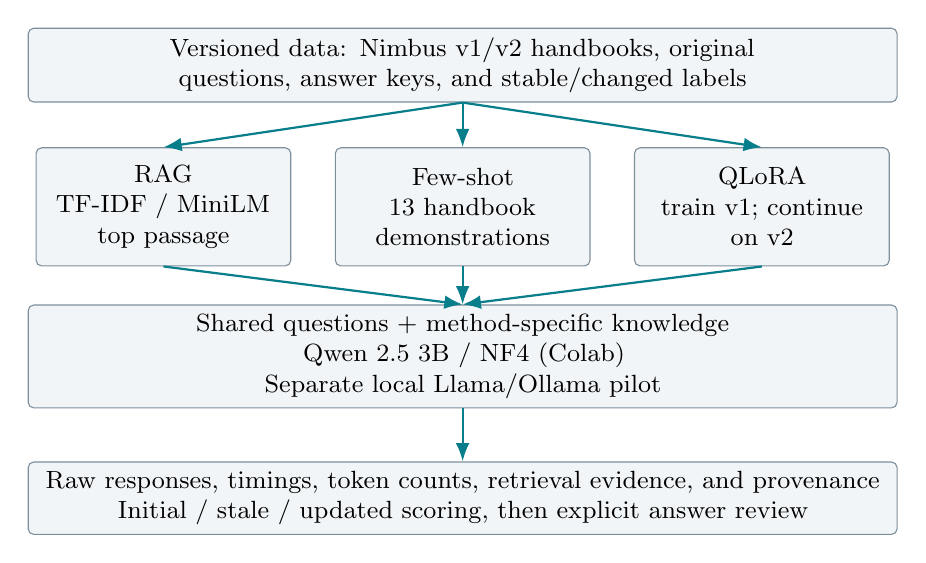
\begin{tikzpicture}[>=Latex,box/.style={draw=navy!55,rounded corners=2pt,fill=light,align=center,font=\small,text width=3.0cm,minimum height=0.9cm},arr/.style={->,thick,teal}]
\node[box,text width=10.8cm] (data) at (0,4.2) {Versioned data: Nimbus v1/v2 handbooks, original questions, answer keys, and stable/changed labels};
\node[box,minimum height=1.5cm] (rag) at (-3.8,2.4) {RAG\\TF-IDF / MiniLM\\top passage};
\node[box,minimum height=1.5cm] (few) at (0,2.4) {Few-shot\\13 handbook\\demonstrations};
\node[box,minimum height=1.5cm] (lora) at (3.8,2.4) {QLoRA\\train v1; continue\\on v2};
\node[box,text width=10.8cm] (model) at (0,0.5) {Shared questions + method-specific knowledge\\Qwen 2.5 3B / NF4 (Colab)\\Separate local Llama/Ollama pilot};
\node[box,text width=10.8cm] (out) at (0,-1.3) {Raw responses, timings, token counts, retrieval evidence, and provenance\\Initial / stale / updated scoring, then explicit answer review};
\foreach \a in {rag,few,lora}{\draw[arr] (data.south) -- (\a.north);\draw[arr] (\a.south) -- (model.north);}
\draw[arr] (model) -- (out);
\end{tikzpicture}}
\caption{Implemented comparative architecture. Zero-shot uses the same base backend with the question and system instruction but no handbook knowledge.}\label{fig:architecture}
\end{figure}

The project persists experiment records as JSON and source documents as Markdown. It does not require a relational database, authentication service, or browser frontend. The command-line interface and notebook are the actual operating interfaces; the figures describe those components rather than a hypothetical web application.

\section{Retrieval and prompting}
The lexical retriever chunks Markdown at level-three headings, fits a scikit-learn TF-IDF vectorizer, and ranks sections by cosine similarity. The dense retriever encodes section text and the question using \texttt{sentence-transformers/all-MiniLM-L6-v2}. Its vectors are normalized, so their dot product gives the similarity used for ranking. Exact search is sufficient for thirteen sections; a separate vector database is unnecessary for this corpus.

Both retrievers return a chunk and a score through the same interface. The generation runner selects the first passage and places it in a policy-context prompt. Few-shot prompting instead adds thirteen user/assistant example pairs before the final question. Zero-shot supplies no handbook material. The shared instruction asks for a concise policy answer and permits an explicit statement of uncertainty.

\section{Model backends and execution}
\texttt{OllamaModel} calls the local server's chat endpoint and retains the returned answer, timing fields, and token counts. HTTP failures propagate as errors rather than being mistaken for model answers. \texttt{HFModel} loads the Qwen model with NF4 quantization, optionally loads a PEFT adapter, and performs deterministic generation with a ninety-six-token output limit. The local and Colab backends share the surrounding data and scoring pipeline, but their performance measurements are not pooled.

The runner iterates over methods, knowledge versions, repeats, and questions. It writes results after each question and marks a run complete only after all requested trials finish. Metadata includes the Git revision, source-file hashes, question and handbook hashes, model settings, environment information, and whether the working tree was dirty. Setup timing is stored separately from per-question timing.

\section{QLoRA training and continued adaptation}
The GPU implementation uses a frozen four-bit base model with trainable low-rank adapters on the query and value projections. The fixed recipe is listed in Table~\ref{tab:training}. Training examples are built from handbook sections rather than the evaluation answer file. Completion-only masking prevents the prompt tokens from contributing to the training loss.

\begin{table}[H]\centering\small
\caption{Fixed QLoRA recipe used for the matched Week~12 sequence.}\label{tab:training}
\begin{tabularx}{\linewidth}{P{0.43\linewidth}L}\toprule
Setting & Value\\\midrule
Base model / hardware & Qwen 2.5 3B Instruct / Tesla T4\\
Training quantization & Four-bit NF4, double quantization, FP16 compute\\
Adapter targets & \texttt{q\_proj}, \texttt{v\_proj}\\
Rank / alpha / dropout & 16 / 32 / 0.05\\
Examples / epochs per stage & 13 / 20\\
Batch size / accumulation & 1 / 4 steps\\
Learning rate / seed & $2\times10^{-4}$ / 42\\
Loss and optimizer & Completion-only loss; AdamW\\
Update initialization & Reload the freshly trained v1 adapter as trainable\\\bottomrule
\end{tabularx}
\end{table}

The following excerpt captures the update operation implemented in \path{finetune/train.py}:
\par\noindent\begin{minipage}{\linewidth}
\begin{lstlisting}[language=Python]
if args.resume_adapter:
    model = PeftModel.from_pretrained(
        model, args.resume_adapter, is_trainable=True)
else:
    model = get_peft_model(model, LoraConfig(
        r=16, lora_alpha=32, lora_dropout=0.05,
        target_modules=['q_proj', 'v_proj'],
        task_type='CAUSAL_LM'))
\end{lstlisting}
\end{minipage}\par
The Week~12 experiment rebuilt v1 and measured it before continuing on v2. This matters because a new adapter cannot be fairly compared with an unrelated older initialization as though they were the same training sequence.

\section{Evaluation records and audit design}
Each evaluation row identifies the method, knowledge version, truth version, question ID, category, question, expected answer, generated answer, and correctness decision. Retrieval rows also record section identity and similarity. A saved original answer appears under both truth versions, but represents one generation.

The paired audit joins v1 and v2 records by question ID, verifies that questions and targets agree, and rejects duplicate or missing IDs. It classifies each fact as gained, lost, stayed correct, or stayed incorrect. Manual corrections are stored separately from raw automatic decisions, with explanatory notes. The published result can therefore be traced back to the response that produced it.

\section{End-to-end example}
For the refund-window question, the local demonstration builds a Version-1 index, retrieves the refund section, and passes that section to the model. The recorded demonstration returns \textbf{30 days}. Rebuilding the index from Version~2 changes the supplied policy passage, and the recorded answer becomes \textbf{45 days}. No model retraining is required for this RAG update.

The repository command is \texttt{python -m experiments.demo ask}. Additional commands display the saved comparative table and inspect an audited answer. This local example demonstrates the input--retrieval--generation--output workflow; the final Qwen accuracy table is supported by its own saved GPU results.

\chapter{Work Achieved During the Semester}
\section{Weeks 1--7: dataset, local pipeline, and initial evidence}
The early work established the research question, the two handbook versions, and the original eleven-fact evaluation. The first implementation was a lexical retrieval and staleness harness. It was extended to MiniLM embeddings and actual generated answers through Ollama, making it possible to distinguish retrieving a useful passage from generating a correct answer.

Few-shot prompting, a zero-shot control, independently worded adaptation examples, and measurement instrumentation completed the local comparison. Three deterministic repeats produced \textbf{231 model generations} and \textbf{363 scoring rows}. The same generated response could be scored against both truths, explaining why the row count exceeds the generation count. Repeated answers were identical in this local pilot; the repeats supplied timing observations rather than additional independent facts.

The early phase also uncovered an evaluation defect. The first scorer accepted the word ``mandatory'' in a rule about administrator accounts as evidence of a mandate for standard accounts. The historical stale changed-fact result of 1/6 was therefore corrected to 0/6. Retaining the original file and recording the correction made the error visible instead of silently replacing the research history.

\section{Weeks 8--9: controlled GPU baselines and initial LoRA}
The Colab study ran TF-IDF RAG, embedding RAG, few-shot, and zero-shot with the same Qwen base model and NF4 inference backend. The retained baseline file contains \textbf{77 generations} and \textbf{121 scoring rows}. The separate original v1 LoRA evaluation added eleven generations and twenty-two scoring rows.

Version-1 QLoRA training completed on a Tesla T4 using thirteen examples and twenty epochs. Its original-truth accuracy was 5/11, and its original answers scored 4/11 when judged against the updated policy. Training and evaluation records captured actual outputs and measurements rather than treating notebook preparation as completed experimentation.

The audit also corrected cases that keyword matching could not settle reliably: ``daily'' was accepted as equivalent to a twenty-four-hour backup interval, and an administrator-only authentication requirement was rejected as evidence of a requirement for all standard accounts. This phase supplied the first model-matched comparison and a clear remaining task: measure the effect of continued v2 training.

\section{Weeks 10--12: matched update and retrieval robustness}
The completed update experiment trained a fresh v1 adapter, evaluated it, continued that same adapter on Version~2, and evaluated the updated adapter. Both generations of results are preserved in a separate Week~12 directory. Eleven paired answers were reviewed against the same v2 target, exposing both learning and regression.

A separate retrieval audit tested word versus character matching and body-only versus title-plus-body indexing. It ran the original and paraphrased questions against both handbook versions. The design produced $11\times2\times2\times4=176$ ranking records. These are repeated observations of eleven facts, not 176 independent questions.

The phase concluded with the audited comparative tables, failure analysis, a LaTeX progress report, a code-and-inference demonstration, and a silent presentation with a read-aloud recording script. The recorded Week~11 finish target slipped into the extended Week~12 reporting period; this report does not retroactively describe that target as having been met on time.

\section{Final repository maintenance and delivery}
Final maintenance added protection against overwriting result files, evidence-consistency checks, adapter archive checksums, a fresh-directory GPU workflow, visible notebook command output, and Linux continuous integration. The repository now contains sixteen passing regression and validation tests. Existing reports remain available as historical milestones, while the README identifies the final results and current commands.

All five project pull requests were merged into \texttt{main} by November~20, with the final maintenance merge recorded as \texttt{a3ba065}. That revision is the code/evidence snapshot used while preparing this report. The final materials include source code, data, raw and audited results, report sources and PDFs, demonstration assets, slides, and a recording script.

Additional November~20 local generation and GPU reproduction attempts were interrupted. They are excluded from the published result tables and are not counted as completed experiments. The completed semester evidence is the preserved local pilot and the Week~8--12 GPU studies.

\chapter{Results and Discussion}
\section{Local pilot: what the first implementation established}
The local Llama/Ollama study established that the full pipeline could generate and score answers under both handbook versions. Table~\ref{tab:local} reports unique-question counts, not the three repeated trials as separate facts.
\begin{table}[H]\centering\small
\caption{Local Llama pilot. The same eleven questions were repeated three times.}\label{tab:local}
\begin{tabularx}{\linewidth}{Lccc}\toprule
Method & Initial & Stale & Updated\\\midrule
TF-IDF RAG & 11/11 & 5/11 & 11/11\\
MiniLM RAG & 11/11 & 5/11 & 11/11\\
Few-shot & 8/11 & 3/11 & 8/11\\
Zero-shot & 0/11 & 0/11 & Not applicable\\\bottomrule
\end{tabularx}
\end{table}
Both RAG methods retained the five stable facts but missed all six changed facts when using stale knowledge. Re-indexing restored the six changed answers. Few-shot prompting made factual errors even though the relevant information was present among its examples. Its matching-version totals were both 8/11, but the specific errors differed.

These local results are not pooled with the Qwen study: the base model, backend, quantization, and hardware differ. Their contribution is evidence that the early end-to-end pipeline worked and that a controlled source update could expose and repair stale answers in this setting.

\section{Final audited Qwen comparison}
Table~\ref{tab:final} is the final comparison. The RAG and few-shot rows use the audited Week~8 baselines; the LoRA row uses the matched Week~12 sequence. Both studies use Qwen 2.5 3B with the same NF4 inference approach, but they are separate recorded sessions. The table is not a claim of one simultaneous randomized benchmark.
\begin{table}[H]\centering\small
\caption{Final core-fact accuracy: original, stale, and updated conditions.}\label{tab:final}
\begin{tabularx}{\linewidth}{Lccc}\toprule
Method & Original & Stale vs.\ v2 truth & Updated\\\midrule
TF-IDF RAG & 10/11 & 6/11 & 11/11\\
MiniLM RAG & 10/11 & 6/11 & 11/11\\
Few-shot & 10/11 & 5/11 & 10/11\\
LoRA, matched sequence & 5/11 & 4/11 & 4/11\\\bottomrule
\end{tabularx}
\end{table}

\begin{figure}[htbp]\centering
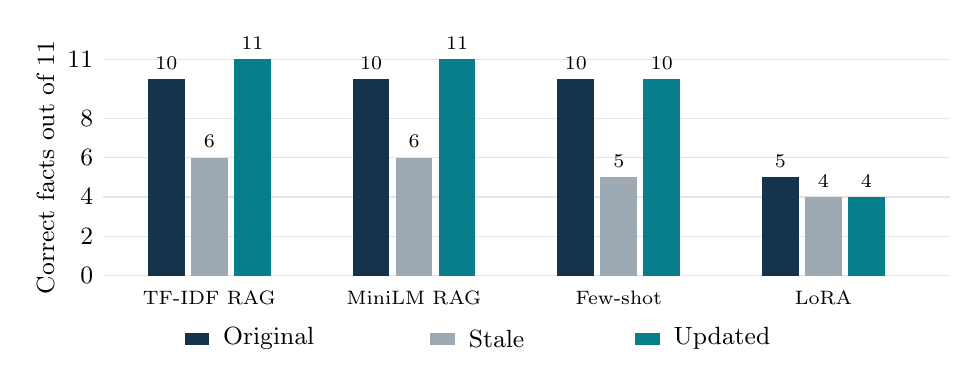
\begin{tikzpicture}[x=0.52cm,y=0.25cm,font=\small]
\foreach \y in {0,2,4,6,8}{\draw[slate!20] (0,\y)--(20.7,\y);\node[left] at (0,\y){\y};}
\node[left] at (0,11){11};\draw[slate!20] (0,11)--(20.7,11);
\foreach \x/\a/\b/\c/\name in {2/10/6/11/TF-IDF RAG,7/10/6/11/MiniLM RAG,12/10/5/10/Few-shot,17/5/4/4/LoRA}{
\fill[navy] (\x-0.9,0) rectangle (\x,\a);
\fill[slate!65] (\x+0.15,0) rectangle (\x+1.05,\b);
\fill[teal] (\x+1.2,0) rectangle (\x+2.1,\c);
\node[above,font=\scriptsize] at (\x-0.45,\a){\a};
\node[above,font=\scriptsize] at (\x+0.6,\b){\b};
\node[above,font=\scriptsize] at (\x+1.65,\c){\c};
\node[below,align=center,font=\scriptsize] at (\x+0.6,-0.3){\name};}
\node[rotate=90] at (-1.4,5.5){Correct facts out of 11};
\fill[navy] (2,-3.5) rectangle (2.6,-2.9);\node[right] at (2.7,-3.2){Original};
\fill[slate!65] (8,-3.5) rectangle (8.6,-2.9);\node[right] at (8.7,-3.2){Stale};
\fill[teal] (13,-3.5) rectangle (13.6,-2.9);\node[right] at (13.7,-3.2){Updated};
\end{tikzpicture}
\caption{The audited comparison. Counts refer to eleven synthetic facts and do not establish statistical superiority.}
\end{figure}

Refreshing either retrieval source yielded 11/11 correct core facts. Few-shot examples yielded 10/11 after refresh. The Qwen zero-shot control scored 1/11 under either truth version, reflecting the accepted daily-backup answer; it had no knowledge-refresh condition. The controlled setting therefore shows the practical value of supplying domain information, while also showing that different mechanisms do not use that information equally reliably under this training and prompt budget.

A stale answer can match the new policy by coincidence. For each RAG method, one changed fact already matched v2 before refresh, and the update corrected the other five. This is why total updated accuracy should not be described as the number of facts newly learned.

\section{LoRA: learning and regression cancel in the total}
The most informative LoRA result is the per-fact transition. The updated adapter learned the sixty-day password-reset interval and ninety-day backup-retention rule. It lost the previously correct Pro Plan specification and the current two-factor authentication requirement.
\begin{table}[H]\centering\small
\caption{LoRA transitions, with both columns scored against Version~2 truth.}\label{tab:transitions}
\begin{tabularx}{\linewidth}{Lrrrr}\toprule
Group & Gained & Lost & Kept correct & Still wrong\\\midrule
Six changed facts & 2 & 1 & 0 & 3\\
Five stable facts & 0 & 1 & 2 & 2\\\bottomrule
\end{tabularx}
\end{table}
Changed-fact correctness rose from 1/6 to 2/6, while stable-fact correctness fell from 3/5 to 2/5. Overall correctness remained 4/11. An unchanged aggregate score therefore concealed both acquisition and regression. The observed regression is consistent with interference during adaptation, but one small training sequence does not establish its general cause or frequency.

The automatic updated score was 5/11 because it credited this answer:
\begin{quote}\small
Two-factor authentication (2FA) is voluntary for standard employee accounts but will be required starting in Q1 2023.
\end{quote}
The v2 policy requires 2FA now. Recognizing the word ``required'' without its temporal context was a false positive. The audit corrected the answer to incorrect, yielding 4/11. The earlier stale answer matched the core mandate but invented SMS-only detail; credit for its core fact did not validate that unsupported addition.

\section{Retrieval robustness under paraphrasing}
All four lexical indexing configurations ranked the correct passage first for all eleven original questions in both handbook versions. Reworded questions exposed differences that those original questions concealed.
\begin{table}[H]\centering\small
\caption{Correct-passage coverage on eleven paraphrases, independent of generation.}\label{tab:rank}
\begin{tabularx}{\linewidth}{Lrrrr}\toprule
 & \multicolumn{2}{c}{Version 1} & \multicolumn{2}{c}{Version 2}\\
Index configuration & Top 1 & Top 3 & Top 1 & Top 3\\\midrule
Word, body only & 6/11 & 7/11 & 7/11 & 7/11\\
Word, title and body & 6/11 & 7/11 & 7/11 & 7/11\\
Character, body only & 8/11 & 10/11 & 8/11 & 10/11\\
Character, title and body & 8/11 & 10/11 & 8/11 & 10/11\\\bottomrule
\end{tabularx}
\end{table}
The character index uses within-word sequences of three to five characters. Adding section titles did not change aggregate hit counts. For the paraphrase about the interval between ``automatic snapshots'' for paying subscribers, the Version-2 word index assigned every passage zero similarity; deterministic document-order tie-breaking placed the correct backup section seventh. Character matching placed it first. For the entry-level plan capacity, the target moved from eleventh to ninth and remained outside the top three.

This experiment supports a narrow finding: character matching improved passage coverage for this paraphrase set. It does not show that supplying three passages improves generated answers. Additional passages could help, introduce distractors, or increase context cost; those outcomes remain to be measured.

\section{Compute measurements and their limits}
The matched Week~12 training stages produced the measurements in Table~\ref{tab:compute}. These are training durations and peak allocated CUDA memory, not total end-to-end project cost.
\begin{table}[H]\centering\small
\caption{Measured training cost for the matched LoRA sequence.}\label{tab:compute}
\begin{tabularx}{\linewidth}{Lrr}\toprule
Stage & Training seconds & Peak allocated GiB\\\midrule
Rebuild Version 1 & 128.2 & 3.36\\
Continue on Version 2 & 128.9 & 3.36\\\bottomrule
\end{tabularx}
\end{table}
Model loading and export are outside these training durations. The data show that the small adapter could be trained within the available T4 memory budget; they do not imply that this training budget was sufficient for reliable policy recall.

In the earlier local CPU-fallback pilot, RAG prompts averaged about 108 tokens, while few-shot prompts averaged about 640--650. Mean local end-to-end times ranged from 1.050 to 1.420 seconds for the two RAG variants across handbook versions, compared with 2.252 and 3.449 seconds for few-shot. These timings came from three deterministic repeats with warm-up excluded. Fixed condition order, prompt caching, different output lengths, and the small workload limit causal conclusions. They must not be compared directly with Colab GPU timings.

\chapter{Testing, Challenges, and Limitations}
\section{Testing and validation evidence}
Testing covered both the experiment logic and final repository maintenance. The initial suite grew from ten checks to twelve after pairing regressions were added, then to sixteen during the final maintenance work. A fresh Python~3.11 macOS environment and Linux GitHub Actions both passed the sixteen-test suite.
\begin{table}[H]\centering\small
\caption{Validation performed and what each result establishes.}
\begin{tabularx}{\linewidth}{P{0.29\linewidth}L}\toprule
Check & What it establishes\\\midrule
Scoring regressions & Numeric boundaries, units, conflicting quantities, concise yes/no answers, scope, and the voluntary-now false positive are handled in tested cases.\\
Retrieval and prompt checks & Original targets can be retrieved; adaptation questions do not copy the evaluation question strings.\\
API failure handling & A model-server failure propagates rather than becoming an answer.\\
Paired-record validation & Question order can change without changing pairing; duplicate IDs cannot conceal a missing fact.\\
Tiny-model gradient check & Completion masking permits finite loss and nonzero adapter gradients. It is not a full-model accuracy test.\\
Adapter archive round trip & A real tiny CPU PEFT adapter can be saved, exported, verified, and reloaded with matching outputs; corruption is rejected.\\
Published-evidence check & The table, explicit overrides, data hashes, unique-question coverage, saved pairs, and 176 rankings agree.\\
Historical live runs & Saved local generations and Colab training/evaluation outputs establish the reported semester experiments.\\\bottomrule
\end{tabularx}
\end{table}

The current CI workflow also executes fresh lexical retrieval and the saved-results demonstration commands. Notebook code cells were parsed, command streaming and failure propagation were checked, and README file links were verified. Passing these checks is narrower than proving correctness for every prompt, every environment, or a production deployment.

\section{Challenges and responses}
\textbf{Limited local compute.} The available Mac had 8~GiB RAM, and the early local run used CPU fallback. A quantized Ollama model enabled local experimentation; CUDA training moved to Colab. The controlled comparison kept the Qwen model and inference backend consistent across its methods.

\textbf{Scoring scope and time.} Keyword matching confused administrator requirements with standard-account requirements, and a future mandate with a current one. The project retained raw outputs, added regression checks, and stored audit corrections separately. This resolved the identified judgments while leaving general semantic scoring as a limitation.

\textbf{Checkpoint continuity and persistence.} The original adapter lacked a verified local backup. The Week~12 comparison therefore rebuilt v1 and continued that same adapter on v2, preserving a matched experiment. The final repository adds a bundle containing both adapters, tokenizer files, results, and checksums. However, the original Week~12 weights still have no verified durable backup. Their hashes identify them but cannot reconstruct them.

\textbf{Evidence preservation.} Reusing output filenames could overwrite historical evidence. The updated runner and training entry point reject existing output locations, and the notebook allocates a fresh run directory. Incomplete runs remain distinguishable from completed evaluations. The interrupted November~20 reproduction attempts are explicitly excluded from the findings.

\section{Limits on the conclusions}
The dataset contains eleven synthetic facts, with only six updates. Training and evaluation intentionally share facts, even though the question strings differ. The results therefore address factual acquisition and retention, not broad language understanding or unseen-domain generalization.

Only one retained matched LoRA sequence supports the reported update analysis. The recipe was not tuned against a separate validation set, and no multi-seed confidence interval is claimed. RAG receives one selected passage while few-shot receives all thirteen demonstrations; equal base models do not imply equal context budgets. The published baseline and LoRA rows also come from different recorded sessions.

The answer audit was assistant-assisted and neither independent nor blinded. Core-fact credit can coexist with unsupported extra detail. Retrieval rankings are not answer-quality measurements, and the 176 rankings are not independent test samples. These limitations are part of the interpretation, not reasons to hide unsuccessful answers.

\chapter{Conclusion and Future Plans}
\section{Summary of what was achieved}
The semester produced the planned three-strategy research pilot. I developed a controlled two-version dataset, implemented lexical and dense retrieval, connected actual model backends, created few-shot and zero-shot conditions, implemented CUDA QLoRA, and measured a matched continued-training sequence. The project also produced explicit answer audits, a paraphrase retrieval study, automated tests, reproducibility documentation, and presentation/report artifacts.

The main practical finding is that updating the retrieval source worked reliably on this handbook: both RAG variants reached 11/11 after refresh. Few-shot prompting reached 10/11. LoRA reached an audited 4/11 after update, with two gains offset by two losses. The per-fact analysis made that unchanged total informative rather than treating it as evidence that nothing changed.

The contribution is the controlled case study, implementation, and failure analysis; it is not a new adaptation algorithm or a universal ranking. The recorded project plan is complete at the pilot level. Larger-scale evaluation, stronger annotation, and production deployment are future work. The final report distinguishes completed measurements from implemented maintenance features whose full GPU rerun was interrupted.

\section{Prioritized future improvements}
\small
\begin{longtable}{P{0.22\linewidth}P{0.34\linewidth}P{0.34\linewidth}}
\caption{Future work and the evidence needed to evaluate it.}\\
\toprule
Priority & Proposed improvement & Success evidence\\\midrule\endfirsthead
\toprule Priority & Proposed improvement & Success evidence\\\midrule\endhead
1. Preserve deployments & Complete a fresh GPU reproduction, export both adapters, verify the downloaded archive, and retain a durable versioned copy. & Successful reload outside the training session, with matching provenance and new recorded responses.\\
2. Expand the evaluation & Add more policies, independent question authors, unseen facts, and multiple update cycles. & Larger held-out evaluation with stable/changed results and uncertainty estimates.\\
3. Strengthen answer review & Use a written scoring rubric and independent, blinded reviewers; distinguish core facts from unsupported additions. & Agreement statistics, adjudicated disagreements, and separate factuality/extra-claim scores.\\
4. Test adaptation stability & Repeat training with multiple seeds and use a validation set for rank, learning-rate, and epoch choices. & Repeated matched sequences, recovery/retention distributions, and a held-out final test.\\
5. Evaluate retrieval changes end to end & Compare word, character, dense, and hybrid retrieval; test top-one versus top-three context. & Generated-answer accuracy, unsupported claims, latency, and token cost on the same questions.\\
6. Improve usability & Add a small comparison interface, answer provenance display, and one-command result inspection. & A demonstrable workflow that exposes the source version and evidence behind an answer.\\\bottomrule
\end{longtable}
\normalsize

Rehearsal examples from stable policies are a candidate way to reduce LoRA regressions, but that is an experiment to conduct rather than an established solution in this project. Similarly, stronger retrieval coverage is a reason to test downstream generation, not a reason to assume that final accuracy will improve.

A broader cost study should measure model load time, indexing, training, update frequency, inference workload, and operational resources on comparable hardware. It should separate one-time setup from repeated use and report energy or dollar cost only when those quantities are actually measured.

\section{Final conclusion}
A policy assistant must be evaluated on both what it learns and what it retains. The completed Nimbus pilot demonstrates that distinction with inspectable code and actual responses. Its strongest result is a reliable retrieval refresh within this small domain; its most revealing failure is an adapter whose unchanged total hides newly learned and newly lost facts. The project provides a working experimental foundation for investigating those trade-offs on a larger and more realistic task.

\appendix
\chapter{Evaluation Set and Answer Audit}
\section{Original facts and answer keys}
\begin{longtable}{P{0.07\linewidth}P{0.38\linewidth}P{0.22\linewidth}P{0.22\linewidth}}
\caption{The complete original evaluation set, with shortened question descriptions.}\\
\toprule ID & Question / fact & Version 1 & Version 2\\\midrule\endfirsthead
\toprule ID & Question / fact & Version 1 & Version 2\\\midrule\endhead
S1 & VPN session timeout & 8 hours & 8 hours\\
S2 & Approved refund processing & 5 business days & 5 business days\\
S3 & Paid-tier backup frequency & Every 24 hours & Every 24 hours\\
S4 & Unresolved ticket escalation & 48 hours & 48 hours\\
S5 & Pro Plan storage and price & 2 TB; \$12.99/month & 2 TB; \$12.99/month\\
C1 & Password-reset interval & 90 days & 60 days\\
C2 & 2FA for standard accounts & Optional; required for admins & Required for all employees\\
C3 & Full-refund request window & 30 days & 45 days\\
C4 & Retention after deletion & 30 days & 90 days\\
C5 & Priority support response & 4 hours & 2 hours\\
C6 & Basic Plan capacity & 100 GB & 150 GB\\\bottomrule
\end{longtable}
Exact questions are in \path{eval/qa_pairs.json}; S/C denote the stable/changed ID prefixes.

\section{Audited LoRA transitions}
Full responses and audit notes are in \path{results/week12/pairs_audited.json}. Scores credit the core fact, not unsupported extra detail.
\begin{table}[H]\centering\small
\caption{All eleven matched answers, scored against Version~2 truth on both sides.}
\begin{tabularx}{\linewidth}{Lll}\toprule
Fact & Stale answer & Updated answer\\\midrule
VPN timeout & Incorrect & Incorrect\\
Refund processing & Incorrect & Incorrect\\
Backup frequency & Correct & Correct\\
Ticket escalation & Correct & Correct\\
Pro Plan & Correct & Incorrect\\
Password reset & Incorrect & Correct\\
Standard-account 2FA & Correct & Incorrect\\
Refund window & Incorrect & Incorrect\\
Backup retention & Incorrect & Correct\\
Priority response & Incorrect & Incorrect\\
Basic Plan & Incorrect & Incorrect\\\bottomrule
\end{tabularx}
\end{table}


\chapter{Installation and Reproduction Guide}
\section{Repository and local verification}
Clone \texttt{main} from the public repository. Current operating details are in the README and \path{docs/REPRODUCIBILITY.md}.

A local verification environment can be created with Python~3.11:
\begin{lstlisting}[language=bash]
git clone https://github.com/Somama12/llm-adaptation-comparison.git
cd llm-adaptation-comparison
python3.11 -m venv .venv
source .venv/bin/activate
python -m pip install -r requirements-train.txt pytest
python -m pip check
python -m pytest -q
python -m experiments.verify_evidence
python -m experiments.demo compare
python -m experiments.demo inspect --id changed_2
\end{lstlisting}
The evidence and comparison commands inspect saved results; they do not train or generate new answers.

For local generation, install and start Ollama, then use new output paths:
\begin{lstlisting}[language=bash]
ollama pull llama3.2:3b
python -m experiments.demo ask
\end{lstlisting}
The reproduction guide gives the full evaluation commands. MiniLM downloads on first use; evaluation outputs require fresh paths.

\section{GPU training and export}
Open \path{notebooks/colab_lora.ipynb} in Colab, select a T4, and run cells in order. Public Qwen needs no token. The workflow invokes:
\begin{lstlisting}[language=bash]
python -m experiments.paired_run \
  --run-dir artifacts/runs/my-new-run
\end{lstlisting}
Use a new run directory. The workflow runs baselines, trains and evaluates v1, continues and evaluates v2, and archives both adapters with tokenizers, results, metadata, and checksums.

Download the ZIP before runtime expiry and verify the local copy:
\begin{lstlisting}[language=bash]
python -m experiments.export_run --verify /path/to/my-new-run.zip
\end{lstlisting}
Adapters require their configured base model. Preserve new outputs separately from Week~12 evidence; fixed seeds do not guarantee identical results across runtime changes.

\chapter{Evidence and Deliverables Index}
\begin{longtable}{P{0.48\linewidth}P{0.43\linewidth}}
\caption{Principal repository artifacts supporting this final report.}\\
\toprule Artifact & Purpose\\\midrule\endfirsthead
\toprule Artifact & Purpose\\\midrule\endhead
\path{data/handbook_v1.md}, \path{data/handbook_v2.md} & Controlled source documents.\\
\path{eval/qa_pairs.json}, \path{eval/qa_paraphrases.json} & Original answer keys and exploratory wording probe.\\
\path{rag/}, \path{experiments/}, \path{finetune/} & Retrieval, prompts, model calls, training, scoring, and result inspection.\\
\path{results/generation_local_scored.json} & Corrected local pilot responses and timings.\\
\path{results/colab_baselines_audited.json} & Audited model-matched baseline answers.\\
\path{results/week12/lora_v1.json}, \path{results/week12/lora_v2.json} & Matched original and updated adapter evaluations.\\
\path{results/week12/pairs_audited.json} & Per-fact transition audit.\\
\path{results/week12/training_v1.json}, \path{results/week12/training_v2.json} & Measured training durations and memory.\\
\path{results/week12/runtime.json} & Recorded GPU package versions and original weight hashes.\\
\path{results/rank_audit.json} & All 176 passage-ranking records.\\
\path{tests/}, \path{.github/workflows/verify.yml} & Regression tests and Linux CI.\\
\path{docs/reports/} & Earlier LaTeX progress reports and PDFs.\\
\path{docs/video/final/} & Recorded code/inference walkthrough, narration, and captions.\\
\path{docs/presentation/} & Silent editable slides and read-aloud recording script.\\
\path{docs/REPRODUCIBILITY.md} & Current setup, export, and reload instructions.\\\bottomrule
\end{longtable}

\textbf{Reading the evidence.} Raw automatic files, explicitly audited files, and retrieval-only outputs serve different purposes. Their names and notes identify those roles. The final comparison combines the audited historical baseline with the matched Week~12 LoRA sequence; incomplete later attempts are not a substitute for either dataset.

\textbf{Reporting scope.} This document covers the completed semester pilot and final maintenance through November~20, 2026. The source code and results were reviewed at revision \texttt{a3ba065}; later report publication does not change the recorded experimental outcomes.
\end{document}
